
\begin{figure}[h]
    \centering
    \begin{overpic}[abs,unit=1mm,scale=.25,width=\textwidth]{fig/baseline_connection_pattern.pdf}
        \put(12,18){\tiny $\hookleftarrow$ PTB} % 在图片上添加公式
    \end{overpic}
    % 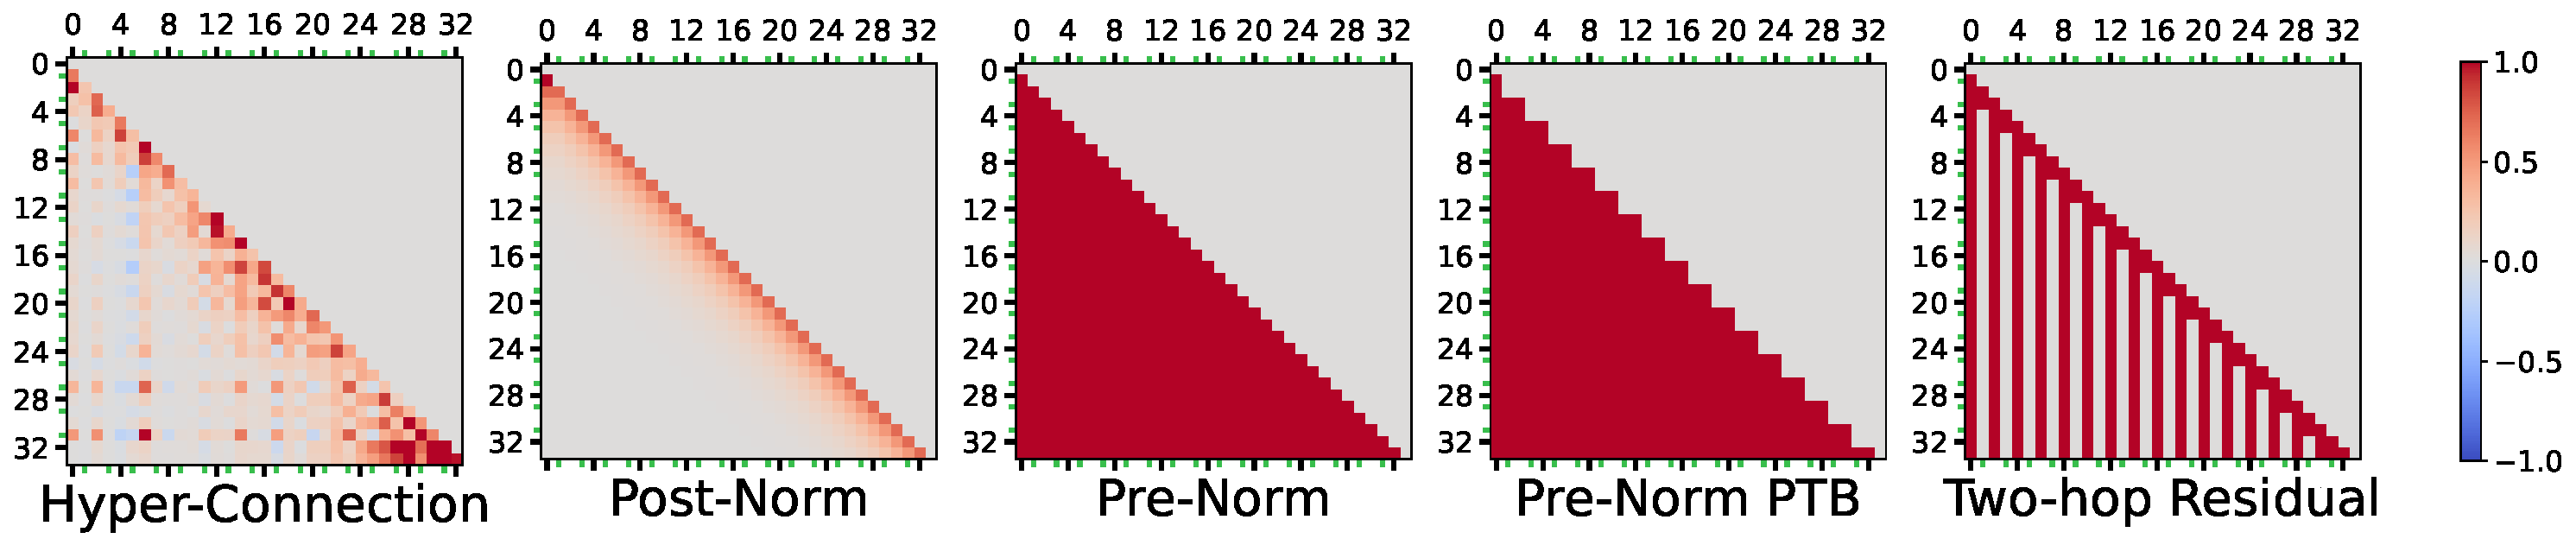
\includegraphics[width=0.98\textwidth]{fig/baseline_connection_pattern.pdf}
    \caption{Visualization of connection matrices for hyper-connections and various related baseline methods. The attention layers, which have odd ids, are marked with green tick marks.}
    \label{fig:compare_connection_pattern}
\end{figure}


In this section, we investigate the learned hyper-connection weights and show how the output of the former layer contributes to the latter ones. To this end, we convert hyper-connections to dense connections cross layers.
Consider the input hidden vectors $\mathbf{h}_0^{k}$ in $k$-th layer, it can be unfolded as a weighted summation over previous layer outputs:
\begin{align}
    \mathbf{h}_0^{k} = \sum_{j=0}^{k-1}{c_{kj}^{(0)}\mathcal{T}^j}(\mathbf{h}_0^{j}),
\end{align}
where $c_{kj}^{(0)}$ describes how much layer-$j$ ($\mathcal{T}^j$) contributes to layer-$k$'s input $\mathbf{h}_0^{k}$. Then, $\mathbf{C}^{(0)}$ denotes a dense connection weight matrix. In particular, let layer-$0$ be the word embedding and $\mathcal{T}^0$ be an identity mapping, layer-$L+1$ be the hidden state before the unembedding layer, which is a summation over the last hidden vectors, i.e., $\mathbf{h}_0^{L+1}=\sum_j \mathbf{h}_j^{L}$. 

\texttt{OLMo-1B-DHC$\times$4} model is adopted for visualization. We take the checkpoint at 500B tokens and forward random validation text to obtain dynamic hyper-connection weights. In addition, we show connection patterns for some related baseline methods. Finally, the visualization is illustrated in Fig.~\ref{fig:1bx4_unfold_connection}. We present the following findings, with more detailed discussions provided in Appendix~\ref{app:more_visulization}.

\textbf{Connection patterns for baseline methods.} For Pre-Norm baseline, the connection matrix is simply a lower triangular matrix with diagonal elements erased, because each transformer layer joins the residual equally. In the Pre-Norm parallel transformer block (PTB) baseline, the connection matrix appears jagged because the input to the FFN layer does not depend on the output of the previous attention layer. For Post-Norm baseline, the connection only holds for adjacent layers, as the weight for bottom layers decays every time the residual passes a post-norm layer. For the two-hop residual baseline~\citep{ma2024megalodon}, the outputs of attention layers are not added to residual and only contributes to the next one FFN layer, resulting in a vertical strip pattern in the connection matrix.

% connection to pre/post norm
\textbf{$\Lambda$-shaped connection pattern. } In the connection matrix for hyper-connections, a long-term decay pattern can be observed, where layers are generally preferred to rely on a few adjacent layer outputs. Moreover, the bottom layers (e.g. layer 0,2) are observed frequently used in most of subsequent layers. Therefore, the two patterns together form a $\Lambda$-shaped connection pattern. Note that the long-term decay pattern is a Post-Norm style pattern, while the frequently accessed pattern is Pre-Norm style, indicating that the hyper-connection introduces a free mixture of Pre- and Post-Norm architecture.

% ideas connection to denseformer
\textbf{Input word embedding is eliminated from model output.} As per the first column in the connection matrix for layer inputs, the input word embedding contributes to most of the layers except for the final one. This last layer, which products the model's output, is used for next token prediction. In most cases, keeping a component of input embedding in model output is harmful to next token prediction, especially when using a tied word embedding such as that employed by \texttt{OLMo-1B}. Similar results are found in previous works~\citep{ma2023denseformer}. % TODO: cite denseformer

% ideas connection to PTB
\textbf{Parallel transformer blocks are observed.} As discussed in \S~\ref{seq_par_dual}, parallel transformer block, which performs attention and FFN in parallel, is a special case for hyper-connection. In practice, PTB-like patterns, which can be identified by the local jagged pattern, are surprisingly observed to be learned by hyper-connections. For instance, layer 11 has a minimal contribution to the input of layer 12 (refer to row 12 in the hyper-connection connection matrix). This suggests that layers 11 and 12 can operate in parallel, thereby forming a PTB module.

% ideas connection to two-hop residual
\textbf{Attention layers tend to have fewer long-term connections.} It is observed that attention layers at the bottom barely have long-term contribution, a trend that persists until layer 17. Upon examining the connection matrix for hyper hiddens (refer to Fig.~\ref{fig:1bx4_unfold_connection} in the appendix), it's evident that the outputs of the FFN layers have significantly greater magnitudes than those of the attention layers. This pattern resembles a two-hop residual connection design, wherein the attention output contributes to the input of the following FFN layer, but doesn't join the main residual path.